\section{Komponentenbeschreibung}
\subsection{Mikrocontroller}
Ein Mikrocontroller ist ein kleiner Computer auf einem einzelnen Halbleiter-Chip. Dazu geh\"ort ein Prozessor,
der Programme ausf\"uhren kann, Arbeits- und Programmspeicher sowie Schnittstellen, die eine Kommunikation mit 
der Umgebung erm\"oglichen sog. Peripheriefunktionen \cite{Wikibooks:2014:Online}. Mit ihnen lassen sich komplexe
Aufgaben l\"osen, f\"ur die sonst ein aufw\"andiger Schaltungsaufbau notwendig w\"are. Standardm\"a{\ss}ig sind folgende Bestandteile in Mikrocontrollern integriert:
CPU, SRAM und Flash-Speicher f\"ur den Programmcode. Weiterhin bieten MCs analoge und digitale Ports, 
mehrere AD/DA-Wandler, Timer und Schnittstellen zur Kommunikation mit der Au\"{ss}enwelt \cite{Viktor:Seib:2014:Online}.
In der nachstehenden Abbildung ist der allgemeine schematische Aufbau eines Mikrocontrollers in folgender Abbildung dargestellt.
\begin{figure}[h!]
	\centering
		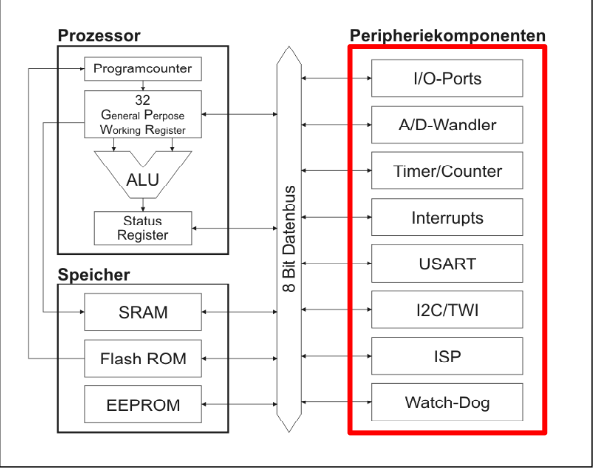
\includegraphics[width=0.9\textwidth]{Aubau_eines_Mikrocontrollers.png}
	\caption{schematischer Aufbau eines Mikrocontrollers \cite{habil:Ostermeye:2014:Online}}
	\label{Aufbau eines Mikrocontrollers}
\end{figure}

\begin{itemize}
\item Prozessor (CPU)
\begin{itemize}
          \item Arithmetic Logic Unit kurz ALU (Rechenwerk)
          \item 32 GPIO-Register (Arbeitsregister f\"ur ALU)
          \item Programmcounter (Programmposition)
					\item Statusregister (Status der aktuellen Operation) 
\end{itemize}
\item Speicher
\begin{itemize}
          \item SRAM Datenspeicher (Static Random-Access Memory)
					\item Flash ROM Programmspeicher (Read Only Memory)
					\item EEPROM Festspeicher (Electrically Erasable Programmable Read-Only Memory)
\end{itemize}
\item Peripheriekomponenten
    \begin{itemize}
          \item I/O-Ports Prim\"arfunktion der Pins (Ein- und Ausg\"ange)
          \item A/D-Wandler (Einlesen von analogen Spannungen)
          \item Timer/Counter (Zeitintervall-/PBM-Generator)
					\item Interrupts (Programmunterbrechungsroutinen)
					\item USART, I2C/TWI und SPI (Kommunikationsschnittstellen)
					\item Watch-Dog (Absicherung gegen Systemfehler)
					\item ISP (Schnittstelle zum \"{U}bertragen des kompilierten Programms)
	\end{itemize}
\end{itemize}
Mikrocontroller sind im heutigen Leben weit verbreitet und es gibt eine viele Anzahl von Herstellern, die mikrocontroller anbieten.
Im folgenden werden einige Hersteller mit ihren MC-Familien beispielhaft aufgef\"urt:
\begin{itemize}
\item Intel (8051-Serie)
\item Renesas (H8)
\item Zilog (Z8)
\item Microchip (Pic)
\item Freescale (fr\"uher Motorola) (68HC08 bzw. 68HCS08)
\item Atmel (AVR, 8051-Serie)
\end{itemize}
F\"ur das Projekt FAISE wurde das Atmel-Serie eingesetzt. Es sind Mikrocontroller mit erweiterten Peripherien und Funktionen, 
die auf der 8-Bit-AVR-Architektur basieren. Bei AVR handelt es sich um einen RISC-Kern, der an der Universit\"at von Trondheim 
in Norwegen entwickelt und von Atmel aufgekauft wurde. Die CPU besitzt 32 allgemeine 8-Bit Register (general purpose registers) 
und ist in der Lage in einem einzigen Taktzyklus Daten aus zwei beliebigen Registern in die ALU zu laden, diese zu verarbeiten 
und das Ergebnis in einem beliebigen Register zu speichern \cite{Viktor:Seib:2014:Online}. Die Konfiguration eines Atmega 8 der Firma Atmel sieht so aus:
\begin{figure}[h!]
	\centering
		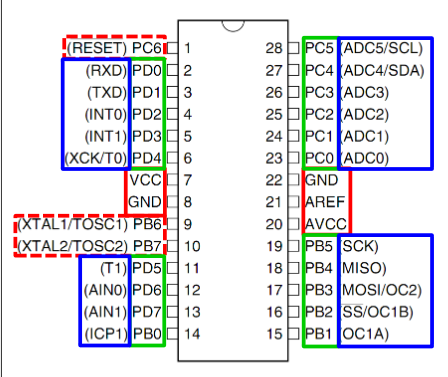
\includegraphics[width=0.9\textwidth]{Atmel8.png}
	\caption{Atmel 8 \\ \url{(http://www.ids.tu-bs.de/tl\_files/Lehre/Vorlesungen/Simulation2/Einfuehrung\_in\_die\_MC\_Programmierung\_Teil1.pdf)}}
	\label{Atmel 8}
\end{figure}
\begin{figure}[h!]
	\centering
		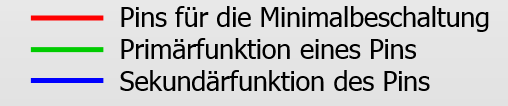
\includegraphics[width=0.9\textwidth]{LegendeAtmel8.png}
	\caption{Atmel 8 \url{(http://www.ids.tu-bs.de/tl\_files/Lehre/Vorlesungen/Simulation2/Einfuehrung\_in\_die\_MC\_Programmierung\_Teil1.pdf)}}
	\label{Legende Atmel8}
\end{figure}
\begin{itemize}
\item Pins f\"ur die Minimalbeschaltung
\begin{itemize}
          \item Spannungsversorgung
          \item ReferenzspannungTaktgeber
          \item Reset      
					\end{itemize}
\item Prim\"arfunktion eines Pins
\begin{itemize}
          \item Ein- bzw. Ausgang
					\end{itemize}
\item Sekund\"arfunktion des Pins
\begin{itemize}
          \item A/D-Wandlereingang
          \item Ext. Interrupt
          \item PBM-Ausgang   
\end{itemize}
\end{itemize}
F\"ur die Programmierung der AVR-Controller gibt es eine kostenlose Entwicklungsumgebung AVR-Studio, die das Einbinden des Compilers problemlos erlaubt.

\subsection{Sensorik/ Aktorik}
Hauptziel der Teilgruppe Materialfluss ist das Management von Paketen auf einer Rampe. Die Aufgabe der Sensorik ist dabei, 
die mit Lichtschranken ausgestatteten Rampen Paketen zu detektieren und auf \"Anderung der Position der Paketen zu reagieren.
Die Lichtschranken bestehen aus einer Lichtstrahlenquelle (dem Sender) und einem Sensor (dem Empf\"anger) f\"{u}r diese Strahlung.
Als Lichtquelle kommt Infrarotlicht zum Einsatz und der Vorteil besteht in der einfachen Einstellung des Sensorsystems durch den
sichtbaren Lichtfleck. Das Funktionsprinzip der Lichtschranke besteht darin, der zu  \"andernden Zustand durch die Lichtintensit\"at mit dem Sensor zu registrieren. 
Die Rampen werden auf Hardwareebene um eine Aktorik zum Arretieren der Kisten erg\"anzt. Diese Aktoren (in unserem Fall die
eingesetzte Bolzenpaar) sind f\"ur das Ausf\"uhren von Bewegungen zust\"andig. Sie sind aktive Stellelemente, die in der 
Antriebs - und Steuerungstechnik, die vom  Mikrorechner angesteuert werden und das Verhalten des Prozesses durch das vom 
Sensor kommende Signal in einer gew\"{u}nschten Weise zu erm\"oglichen. In dieser allgemeinen Darstellung stehen die 
Ausgangssignale eines Sensors und die Stellsignale der Aktoren mit einem
Informationsverarbeitungssystem (IVS) in Verbindung.

\subsection{Contiki}
Contiki ist ein Open Source Echtzeitbetriebssystem, das bei uns in der PG auf den MICAz-Modulen eingesetzt wird.
Contiki bietet einen einfachen ereignisgesteuerten Betriebssystemkern mit sogenannten Protothreads, optionalem 
pr\"aemptiven Multiprogramming, Interprozesskommunikation via Messagepassing durch Events, eine dynamische Prozessstruktur
mit Unterst\"utzung f\"ur das Laden und Entladen von Programmen, nativen TCP/IP-Support \"ber den uIP TCP/IP-Stack und eine 
grafische Benutzerschnittstelle, welche direkt auf einem Bildschirm oder als virtuelle Anzeige \"uber Telnet oder VNC genutzt werden kann \cite{Wikipedia:2013:Online}.
 
\subsubsection{Systemarchitektur}
Ein laufendes Contiki System besteht aus dem Kernel, Bibliotheken, Prozessen und dem Programm-Lader, mit dem Anwendun-
gen zur Laufzeit aus dem Speicher oder \"uber ein Funkmodul geladen werden k\"onnen. Die unter stehende Abbildung zeigt die Aufteilung des Betriebssystems in zwei Teile. 
\begin{figure}[h!]
	\centering
		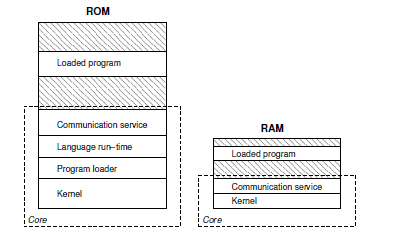
\includegraphics[width=0.9\textwidth]{Systemarchitektur_Contiki.png}
	\caption{Adam Dunkels, Bj\"orn Gr\"onvall, Thiemo Voigt: Contiki - a Lightweight and Flexible Operating System for Tiny Networked
	Sensors. \url{(Quelle:http://www.up.edu.ps/ocw/upinar/moodledata/872/moddata/assignment/970/1287/10.1.1.59.2303.pdf)}}
	\label{Systemarchitektur von Contiki}
\end{figure}
Der Core ist ein Basissystem und besteht aus dem Kernel, Bibliotheken, Ger\"{a}tetreiber und der Programm-Lader. 
Im allgemeinen sind \"Anderungen am Core nicht vorgesehen und nur unter Verwendung eines speziellen Bootloader m\"oglich. 
Die konkrete Aufteilung des Systems in Core und ladbare Programme wird beim Kompilieren des Systems entschieden und h\"angt 
von der Hardware-Plattform ab \cite[S. 7]{Walter:2010}. Ger\"atetreiber werden als Bibliotheken implementiert. 

\subsubsection{Events}
In Contiki kommunizieren Prozesse \"uber Events. Auch der Kernel versendet Events, um Prozesse \"uber ihren Status 
(Init, Continue, Exit) oder \"uber abgelaufene Timer zu Informieren. Zur Identifikation stehen dabei Event IDs zur 
Verf\"ugung. Die Event IDs 0-127 k\"onnen vom Benutzer frei vergeben werden, w\"ahrend die Prozess IDs ab 128 vom 
System genutzt werden. Grunds\"atzlich unterscheidet Contiki zwischen synchronen und asynchronen Events. 
\begin{itemize}
\item Asynchronen Events
\end{itemize}
Asynchrone Events sind eine Form der Deferred Procedure Call: asynchrone Events werden vom Kernel in einer 
Warteschlange gespeichert. Die Scheduling-Funktion des Kernels l\"auft nach Systemstart in einer Endlosschleife. 
In jedem Durchlauf wird ein Event aus der Schlange entnommen und wird einige Zeit sp\"ater an den Zielprozess weitergeleitet.
\begin{itemize}
\item Synchronen Events
\end{itemize}
Synchrone Events gleichen einem Funktionsaufruf. Die werden ohne Umweg \"uber die Warteschlange direkt an den Empf\"anger-Prozess
zugestellt \cite[S. 7]{Walter:2010}.  Mit der Funktion process\_post\_synch(\&example\_process, EVENT\_ID, msg) wird gezielt ein 
Prozess aufgerufen (ein Broadcast ist nicht m\"oglich). W\"ahrend der aufgerufene Prozess aktiv ist, blockiert der Aufrufer und 
setzt seine Ausführung erst fort, wenn der aufgerufene Prozess die Kontrolle wieder abgibt.

\subsubsection{Prozesse}
Prozesse in Contiki implementieren ein Konzept namens Protothreads. Dies erlaubt es Prozessen, ohne den Overhead und die langen 
Prozesswechselzeiten von normalen Threads auszukommen. Gleichzeitig k\"onnen trotzdem andere Prozesse ausgef\"uhrt werden, falls
ein Prozess auf ein Event (Timer, Nachricht von anderem Prozess...) warten muss. F\"ur die Entwicklung mit Prozessen ist wichtig, 
dass nicht-statische Variablen nicht zwischen zwei Aufraufen erhalten bleiben. Der relevante Status eines Prozesses sollte daher 
mithilfe von statischen Variablen abgelegt werden (siehe Variable i im folgenden Beispiel:

\begin{figure}[h!]
	\centering
		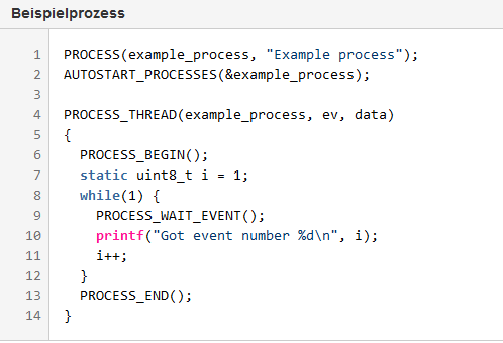
\includegraphics[width=0.9\textwidth]{Beispielprozess.png}
	\label{Beispielprozess}
\end{figure}
In Zeile 1 wird der Prozess initialisiert und in Zeile 2 automatisch beim Boot von Contiki gestartet. Zeile 4 beinhaltet die
Deklaration. So k\"onnen andere Prozesse diesem Prozess Events (mit oder ohne Daten) schicken, auf die unser Beispielprozess 
mit ev und data zugreifen kann. Zeile 6 kennzeichnet den Beginn der tats\"achlichen Ablauflogik. Code \"uber dieser Zeile wird 
bei jedem Prozessaufruf ausgef\"uhrt, dies wird jedoch in den meisten F\"allen nicht ben\"otigt. Zeile 13 schlie{\ss}lich beendet
den Prozess und entfernt ihn aus der Prozess-Liste des Kernels. In diesem Beispiel wird die Zeile jedoch nie erreicht, sodass er
Prozess immer wieder aufgerufen wird, bis er von einem anderen Prozess beendet wird.
Wichtige Funktionen in Prozessen:
\begin{itemize}
\item PROCESS\_WAIT\_EVENT()- Wartet auf ein beliebiges Event, bevor die Ausf\"{u}hrung fortgesetzt wird
\item PROCESS\_WAIT\_EVENT\_UNTIL(condition) - Wartet auf ein beliebiges Event, setzt die Ausf\"{u}hrung aber nur fort, wenn die Bedingung erf\"{u}llt ist
\item PROCESS\_WAIT\_UNTIL() - Wartet, bis die Bedingung erf\"ullt ist. Muss den Prozess nicht zwangsl\"{a}ufig anhalten
\end{itemize}
Prozesse k\"onnen \"uber Events (siehe Events) oder Polling-Anfragen kommunizieren.  Polls sind Events mit hoher Priorit\"at und 
k\"onnen genutzt werden, um den angerufenen Prozess so schnell wie m\"oglich auszuf\"uhren. Sie
sind besonders bei der Abarbeitung von Hardware-Interrupts wichtig, da Interrupts-Handler keine Events, sondern nur
Polling-Anfragen absetzten d\"urfen \cite[S. 7]{Walter:2010}.